\chapter{\section{\mbox{Introduction}}{\normalfont\fontsize{14}{16}\bfseries}}
\label{introduction}
It was the capacity of labor that propelled humanity forward, shaping the evolution of civilization and moulding its contours. In the modern world contemporary societies emerged as hybrid environments where the physical world intertwined seamlessly with digital. Human interaction found new means when virtual communication got advanced, while artificial intelligence is standing shoulder to shoulder with natural intelligence. 

The tools are also being evolved at this time. The tools are no longer bounded in human hands and they are not guided solely by human will. Artificial intelligence enabled autonomy for these tools granting the machines the power to operate independently, make decisions, and chart their own course. As the world stood on the edge of this paradigm shift, the need for a deeper understanding of this technology became important.

Researchers, policymakers businesses, and society at large, all joined hands recognizing technology in all its brilliance,must remain a servant to humanity. The tool must enhance work preserving its current dual nature well spring for creation and a conduit for human fulfillment. After the pandemic COVID-19 hit the world the evolution of automation and AI was accelerated, reshaping warehouses, manufacturing plants, grocery stores, and call centers. The emergence of artificial intelligence rewrote the structure of human life transferring the way we were toiled, the way we learned and the way we structured our businesses and work. The world of robotics and automation ushered in a new era of collaboration. Man and machine are now sharing tasks, space, and even rhythm of creation.\cite{author1}
 
 Four repeated modes of collaboration of humans and robots emerged, These modes are named  co-existence, sequential collaboration, co-operation, and responsive collaboration complimenting each other's strength as shown in Figure\ref{Fig:1l}.
 \begin{figure}[H]
    \centering
    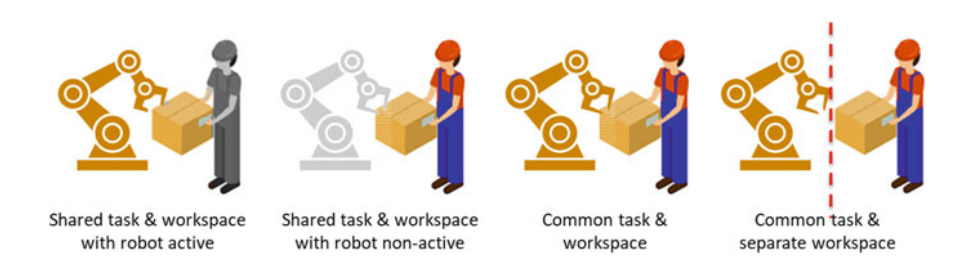
\includegraphics[width=0.8\linewidth]{Figures/Human Robot collaboration.png}
    \caption{Types of Human Robot Collaboration in industrial environment\cite{author3}}
    \label{Fig:1l}
\end{figure}
As the wheel of progress is spinning faster robotics and AI is being advanced in tandem with Big Data, Industry 4.0, and the Internet of Things. The possibilities expanded, expanding far beyond the repetition of modes, technical configurations multiplied, each tailored to the specific demands of tasks, robots, collaboration styles, and production domains.

The integration of collaborative robot systems is a significant leap forward in industrial environments. With careful consideration of the human element, organizations can harness the full potential of this technology, redefining how humans and robots collaborate for increased productivity and safety.

 The International Organization of Standardization (ISO) defines a robot as an “automatically controlled, reprogrammable multipurpose manipulator, programmable in three or more axes, which can be either fixed in place or mobile for use in industrial automation applications” .\cite{author2}
 
 The emerged hybrid production systems aim to alleviate stress and workload blending the strengths of humans and robots. Safety became the cornerstone as robots gained the ability to sense and respond to their environment. Robots can now detect the touch of human hands, adapt to the presence of human workers and even anticipate their motions and conversations by integration of AI in robotics enhancing the safety of Human robot interaction. 
 
 Human-robot interaction is a critical aspect of collaborative robot systems. It encompasses verbal and non-verbal communication, visual information, and gestures, all of which contribute to effective collaboration. In manufacturing, where tasks are often iterative and involve physical interaction, compliance with human states and intent is paramount. While substantial progress has been made in safety within Human robot interaction, challenges remain, particularly in achieving predictability. Designing robots to be tools that humans can understand and control is crucial. This requires formal conditions for system observability and controllability, as well as an understanding of the human's ability to control complex systems.\cite{author3}

While EN ISO 10218 part 1 and 2  were amended in 2011 there were safety measures suggested for human-robot collaboration in the collaborative cell this lead to an exponential rise in the research area of HRC.
Later in ISO/TS 15066, the limiting of forces in different type of robot movement and the design of the robot cells in a safe way were described for collaborative operations of robot with human, but AI integration and introducing cognitive abilities for a collaborative robot is not encompassed in this standards and technical specification.

The research questions we try to address through this thesis are 
What are the potential safety risks associated with AI-Integration in human-robot collaborative environments? How do AI-driven systems interact with other robotic functionalities, and what are the implications for overall system performance? What could be a risk analysis technique for AI-integrated robotic systems? What measures can be taken to ensure seamless integration of AI into lightweight cobots?

We try to answer these questions by studying perception and perception-based application in robotics.
Perception is one technology that is integrated into the robots, which enables the robots to understand their surroundings. Perception allows the robot to identify work material, human co-workers and the dynamic environment in which the robot is. AI-based grasping is one collaborative operation of the robot which can be derived from perception. The robot can grasp an object and pass to humans or humans can work on one object and then the robot picks it up or vice versa.

A process Failure Mode Effective Analysis on AI-based grasping is done in this thesis extending it with System Theory Process Analysis. AI-based grasping algorithms are studied and possible failures of these algorithms are viewed.The Hazard and Risk assessments are based on ISO/TS 12100, keeping in mind the EN ISO 10218-1,2:2011 and the technical specification ISO/TS 15066. 

To increase the reliability of the perception algorithm that induces grasping, different methods are proposed as the result of the thesis. In light of the results from this analysis of risk and hazards a safety framework is formulated for AI-based grasping, which can be taken into consideration, for a generic safety standard for the integration of artificial intelligence in robots.
